\documentclass[conference]{IEEEtran}
\IEEEoverridecommandlockouts
% The preceding line is only needed to identify funding in the first footnote. If that is unneeded, please comment it out.
\usepackage{cite}
\usepackage{amsmath,amssymb,amsfonts}
\usepackage{algorithmic}
\usepackage{graphicx}
\usepackage{textcomp}
\usepackage{xcolor}
\usepackage{braket} %braket notation
\usepackage[ruled,norelsize]{algorithm2e} %algorithm
\usepackage{makecell}
\usepackage{url}
\usepackage{hyperref}
%newtheorem
\newtheorem{definition}{Definition}
%new commands
\DeclareMathOperator*{\argmin}{arg\,min}
\DeclareMathOperator*{\argmax}{arg\,max}

\def\BibTeX{{\rm B\kern-.05em{\sc i\kern-.025em b}\kern-.08em
    T\kern-.1667em\lower.7ex\hbox{E}\kern-.125emX}}

% H specifier 
\makeatletter
\newcommand{\removelatexerror}{\let\@latex@error\@gobble}
\makeatother



%--------------------------------------------------------------------------
% Main document
\begin{document}
\title{Non-linear Constrained Optimization Problem using Byzantine Distributed Optimization Algorithm\\
Group 15 Final Report\\
% {\footnotesize \textsuperscript{*}Note: Sub-titles are not captured in Xplore and
% should not be used}
% \thanks{Identify applicable funding agency here. If none, delete this.}
}




\author{\IEEEauthorblockN{1\textsuperscript{st} Ming-Yu Chung}
\IEEEauthorblockA{\textit{Department of Electrical Engineering} \\
\textit{National Taiwan University}\\
Taipei, Taiwan \\
r11921043@ntu.edu.tw}
\and
\IEEEauthorblockN{2\textsuperscript{nd} Po-Yu Chen}
\IEEEauthorblockA{\textit{Department of Electrical Engineering} \\
\textit{National Taiwan University}\\
Taipei, Taiwan \\
r11921a15@ntu.edu.tw}}



\maketitle

%--------------------------------------------------------------------------------
%Abstact
\begin{abstract}
The constrained optimization problem is an important topic nowadays. An efficient algorithm of the constrained optimization algorithm is crucial in many fields, such as applied mathematics, signal processing, computer science, etc. One of the most famous algorithms is linearization method. However, we notice that the linearization method would  produce terrible outcomes when some parts of functions or constraints in the optimization problem are unsuitable for linear approximation, especially for those who are non-linear. This would lead to a extremely small step size. To deal with this problem, in this report, we develop an algorithm based on linearization method and Byzantine distributed optimization algorithm to solve non-linear constrained optimization problems. 

Our algorithm proposed in this report is constructed as follows. We first introduce a novel idea. We extend the definition of ``fault" in the Byzantine distributed optimization problem and then use the Byzantine distributed optimization algorithm (BDOA) as a filter. The BDOA would identify which functions or constraints is suitable for linear approximation and hence divide the optimization problem into two parts. For the part that constraints are suitable for linear approximation, we use linearization method; for the part that constraints are unsuitable for linear optimization, we use the proximal point method. 

We also perform a series of experiments to demonstrate that our algorithm is more efficient compared to linearization method. The experimental results show that our algorithm is experimental better than linearization method.
\end{abstract}

\begin{IEEEkeywords}
Non-linear constrained optimization; constrained optimization; Distributed optimization; Approximate fault-tolerance; Distributed gradient-descent
\end{IEEEkeywords}

%------------------------------------------------------------------------------------
%Introduction
\section{Introduction}
Constrained optimization problem is an important and critical topic for many fields, like applied mathematics, signal processing, computer science, etc. Many problems in different fields can be transformed as a constrained optimization problem. Take support vector machine (SVM) for example. Given a function class $\mathcal{H}= \{f_{\theta}: \mathcal{X} \rightarrow \mathcal{Y} | \theta \in \Theta \}$, distribution $\mathcal{D}$, dataset $D=\{(x, y)| x\in\mathcal{X}, y\in\mathcal{Y}, (x, y)\sim \mathcal{D}\}$, a constrained function $C_i: \mathcal{H} \times (\mathcal{X}, \mathcal{Y}) \rightarrow \mathbb{R}$ where $i=1\sim n$. The support vector machine (SVM) problem can be expressed as an optimization problem. That is, 
\begin{equation*}
\tag{SVM}
\begin{cases}
    \argmin_{\theta\in\Theta} \|\theta\|^2 \\
    \text{subject to }
    \mathbb{E}_{(x, y) \sim \mathcal{D}} ~C_i(f_{\theta}, (x, y)) \leq 0, ~\forall{i\in[n]}.
\end{cases}
\label{ml1}
\end{equation*}
Since the distribution $\mathcal{D}$ is unknown for almost all cases, we usually simulate \eqref{ml1} as follows:

\begin{equation*}
\tag{SVM*}
\begin{cases}
    \argmin_{\theta\in\Theta} \|\theta\|^2 \\
    \text{subject to }
    \frac{1}{|D|}\sum_{(x, y) \in D} C_i(f_{\theta}, (x, y)) \leq 0, ~\forall{i\in[n]}.
\end{cases}
\label{ml2}
\end{equation*}
By \textbf{law of large numbers}, we can ensure that the solution of \eqref{ml2} would converge to \eqref{ml1} in probability as $|D|\rightarrow \infty$. 

The optimization problem \eqref{ml2} is a typical constrained optimization problem. There are so many optimization algorithms to solve such a constrained optimization problem. One of the most well-known algorithms is \textbf{linearization method} \cite{wilson2012linearization}. 
However, if some parts of the constraints are too complicated, especially for non-linear constraints, the linearization method may perform terribly. To deal with this problem, in this report, we develop a constrained optimization algorithm based on \textbf{linearization method} and \textbf{Byzantine distributed optimization algorithm}. The details of linearization method and Byzantine distributed optimization algorithm would be explained in the section \ref{BKRW}.

The main idea of our algorithm is that we want to utilize the Byzantine distributed optimization algorithm to filter the constraints which are unsuitable for linear approximation. For the constraints suitable for linear approximation, we use linearization method; for the constraints unsuitable for linear optimization, we use the proximal point method. We expect that our method would perform better than linearization method for the cases where some constraints are non-linear. 

Following are our main contributions in this report:
\begin{itemize}
    \item We extend the definition of ``fault" in the Byzantine distributed optimization problem. Then, we utilize the Byzantine distributed optimization algorithm as a filter to identify the constraints which are unsuitable for linear approximation.
    
    \item We develop an algorithm based on linearization method and Byzantine distributed optimization algorithm to deal with non-linear constrained optimization problems. We expect our algorithm to solve the problem more efficiently than linearization method.

    \item We perform some experiments to demonstrate the advantage of our algorithm compared with linearization method.
\end{itemize}


%------------------------------------------------------------------------------
%Background knowledge and related works
\section{Background knowledge and related works}\label{BKRW}
In this section, we would first talk about previous works. Then, we would briefly introduce \textbf{Byzantine distributed optimization problem} and \textbf{Linearization method} which are important components of this report. Besides, we would also define the \textbf{constrained optimization problem} where we are interested in this report.

\subsection{Previous works}
In this report, what we are doing is hybrid two kinds of optimization algorithms to generate a better one. The most similar works are \cite{li2010hybrid, xu2022resilient}. The first one talks about how to hybrid two kinds of algorithms, an \textbf{improved genetic algorithm (IGA)} and an \textbf{improved particle swarm optimization (IPSO)}. The second one talks about how to apply Byzantine distributed optimizations to solve constrained optimization problems. However, no one ever researches how to hybrid Byzantine distributed optimization algorithm and constrained optimization algorithm to develop a more efficient constrained optimization algorithm. So, what we are doing is a very novel topic. 

 
\subsection{Byzantine distributed optimization problem}
The Byzantine distributed optimization problem which we consider in this report can be described as following settings:
\begin{itemize}
    \item \textbf{Agent}: There are m agents. For $i$-th agent, he holds a cost function $C_i:\mathbb{R}^n \rightarrow \mathbb{R}$. The $i$-th agent will also send the information of his cost function to the central server according to the order from the central server.  We say the $i$-th agent is a Byzantine faulty agent if he sends incorrect information to the central server. Otherwise, we call him an honest agent.
    \item \textbf{Central server:} Central server aims to utilize the information obtained from each agent to solve the following optimization problem:
    \begin{align}
    \argmin_{x\in \mathbb{R}^n} \sum_{i\in\mathcal{H}} C_i(x), \label{bdop}
    \end{align}
    where $\mathcal{H}$ is the index set of honest agents and $\mathcal{B}$ is the index set of Byzantine faulty agents.
\end{itemize}

Byzantine distributed optimization problem is defined as the optimization problem \eqref{bdop} under the above settings. It is worth to mention that \cite{su2016fault, gupta2019byzantine1, gupta2019byzantine2, liu2021approximate} have shown that 
\textit{``The exact fault tolerance problem \eqref{bdop} cannot be solved without some specific condition ($2\mathcal{B}$-redundancy)".} The $2\mathcal{B}$-redundancy is defined as following:
\begin{definition}[$2\mathcal{B}$-redundancy]\label{2bred}
We say that the Byzantine distributed optimization problem satisfies $2\mathcal{B}$-redundancy if the number of the honest agents is two times more than the number of the Byzantine faulty agents. That is, 
\begin{equation}
    |\mathcal{H}| \geq 2|\mathcal{B}|.
\end{equation}
\end{definition}
Hence, in this project, we always assume $2\mathcal{B}$-redundancy is satisfied. 

On the other hand, the algorithm solving Byzantine distributed problem is called \textbf{Byzantine distributed optimization algorithm (BDOA)}. 
One of the most famous BDOA is \textbf{Gradient-Filter-based Distributed Gradient Descent}, whose key idea is to mitigate the detrimental impact of incorrect gradients. Following is the related works of this kind of BDOA: comparative gradient elimination (CGE) \cite {gupta2020byzantine3}, coordinate-wise trimmed mean (CWTM) \cite {su2016fault}, geometric median-of-means (GMoM) \cite {chen2017distributed}.


\subsection{Setting of the constrained optimization problem and our goal}
After defining the Byzantine distributed optimization problem, we start to define the constrained optimization problem, which we consider in this report.
In this project, we want to develop an algorithm to solve the following constrained optimization problem:
\begin{equation*}
\tag{P0}
\begin{cases}
    \argmin_{x\in \mathbb{R}^n} &C_0(x)\\
    \text{subject to} &C_i(x) \leq 0, \text{ where } i \in [m],
\end{cases}
\label{P0}  
\end{equation*}
where $C_i(x):\mathbb{R}^n \rightarrow \mathbb{R}$, for any $i = 0\sim m$.

In a practical situation, we would approximate \eqref{P0} as:
\begin{equation*}
\tag{P0*}
\begin{cases}
    \argmin_{x\in \mathbb{R}^n} &C_0(x) + 
    \sum_{i \in [m]} k\cdot\text{ReLU}(C_i(x)),\\
\end{cases}
\label{P0*}  
\end{equation*}
where $k>0$ and the solution of \eqref{P0*} tends to the solution of \eqref{P0} as $k\rightarrow\infty$.
Notice that \eqref{P0*} is similar to the form of Byzantine distributed optimization problem \eqref{bdop}. For convenience, in this report, we would not distinguish \eqref{P0*} and \eqref{P0} and utilize \eqref{P0*} to relate the BDOA.

In this report, we utilize the technique of BDOA to enhance the performance of some existing constrained optimization algorithms on \eqref{P0}. To be more specific, we want to improve linearization method. \cite{wilson2012linearization}. The details of linearization method would be discussed in the next subsection.

\subsection{Linearization method}
As we have mentioned, linearization method is an algorithm for constrained optimization problem \eqref{P0}. In this subsection, we would introduce the linearization method in detail according to \cite{wilson2012linearization}. The convergence analysis is not included in this report but the corresponding proof can be found in \cite{wilson2012linearization}.

Just like the literal meaning, the main idea of linearization method is `` linearize all functions in the constrained optimization problem \eqref{P0}". Given a smooth function $f: \mathbb{R}^n \rightarrow \mathbb{R}$. According to the Tyler expansion, we can express $f$ as a linear approximation as follows:
\begin{equation}
    f(x+p) =  f(x) + \braket{\nabla f(x), p} + O(\|p\|^2),\label{linap}
\end{equation}
where $p$ is some unit direction in $\mathbb{R}^n$. Based on this, at first, we utilize \eqref{linap} to linearize the constrained optimization problem \eqref{P0}. We can obtain follows:
\begin{equation*}
\begin{cases}
    \argmin_{p} &C_0(x) + \langle \nabla C_0(x), p\rangle \\
    \text{subject to} &C_i(x) + \langle \nabla C_i(x), p\rangle \leq 0, \text{ where } i \in [m].
\end{cases}
\end{equation*}
Notice that the linear approximation is only valid when $\|p\|^2$ is sufficiently small. We must add some regularization terms in the optimization problem to avoid $\|p\|^2$ being too large. That is, we transform the optimization problem as follows:
\begin{equation*}
\tag{P1}
\begin{cases}
    \argmin_{p} &C_0(x) + \langle \nabla C_0(x), p\rangle +  \|p\|^2\\
    \text{subject to} &C_i(x) + \langle \nabla C_i(x), p\rangle \leq 0,\forall i \in [m].\label{P1}
\end{cases}
\end{equation*}
Then, what linearization method does is solve \eqref{P1} iteratively to obtain the solution of \eqref{P0}, which can be expressed as \textbf{Algorithm} \ref{linerarization}.
\begin{figure}[htbp]
 \removelatexerror
  \begin{algorithm}[H]
   \caption{Linearization method}
   Given an initial point $x^0 \in \mathbb{R}^n$, $\epsilon > 0$, $N>0$ and iteration number $I$\;
   \For{$k := 0$ to $I$}
   {
      $p^k \gets \text{ the solution of }$ \eqref{P1} at $x = x^k$\;
      $\alpha^k\gets\alpha(x^k, p^k, \epsilon, N)$\;{\color{blue}\tcp{$\alpha$ is defined at the bottom}}
      $x^{k+1}\gets x^k + \alpha^k \cdot p^k$\;
      $k\gets k+1$\;
   }
   \Return{$x^k$}\newline

   {\color{blue} 
   \tcp{
   The function $\alpha(x^k, p^k, \epsilon, N)$ is defined as the minimum $i$ such that following inequality holds:
   \begin{align*}
   C_0(x^k + (\frac{1}{2})^i p^k) + NF(x^k + (\frac{1}{2})^i p^k)
   &\leq  \\
   C_0(x^k) + NF(x^k) - (\frac{1}{2})^i\epsilon\|p^k\|^2,
   \end{align*}
   where $F(x) = \max_{i\in\{0,1,\dots, m\}} C_i(x)$. }}
   \label{linerarization}
  \end{algorithm}
\end{figure}

When the functions $C_i(x)$ have some good properties like convex, Lipschitz continuous, etc, we can ensure the output of \textbf{Algorithm} \ref{linerarization} would converge to the solution of the optimization problem \eqref{P0}. More details and the convergence analysis are also discussed in the \cite{wilson2012linearization}.

\section{Proposed algorithm}
In the previous section, we briefly introduced the critical components of our proposed algorithm. Now, in this section, we would explain how to develop an algorithm for non-linear constrained optimization problems \eqref{P0}, which is based on \textbf{linearization mehod} and \textbf{Byzantine distributed optimization algorithm (BDOA)}.

\subsection{Observation on linearization method}
First of all, we observe the linearization method (\textbf{Algorithm} \ref{linerarization}). There are two important values in the algorithm, descent direction $p^k$ and step-size $\alpha^k$. When some parts of the functions $C_i(x)$ in \eqref{P0} are not suitable for linear approximation, the $\alpha^k$ will be very close to zero. Then, the linearization method would perform inefficiently due to
\begin{equation*}
    x^k + \alpha^k \cdot p^k \approx x^k + 0.
\end{equation*}
Inspired by this drawback of the linearization method, we figure out a method to cope with this problem of linearization method. We think that we should divide \eqref{P0} into two parts. For the part which is suitable for linear approximation, we use the linearization method to optimize; For the part where linear approximation performs terribly, we use another optimization algorithm. Thus, in order to realize our idea, we must need to construct a filter to identify which function $C_i(x)$ is suitable for linear approximation. In the next subsection, we will explain how we achieve this goal by BDOA.

\subsection{Using the BDOA as a filter}
Recall the definition of the Byzantine distributed optimization problem \eqref{bdop}, we notice that BDOA can only optimize on the $C_i(x)$ which belongs to honest agents. The BDOA performs as a filter that identifies the index set of honest agents $\mathcal{H}$ and then only optimizes on the corresponding $C_i(x)$. Hence, if we can consider ``unsuitable for linear approximation" as a fault in Byzantine distributed optimization problem, the BDOA will identify the index set of honest agents $\mathcal{H}$ automatically during the process of optimization.

Given a smooth function $f:\mathbb{R}^n \rightarrow \mathbb{R}$. Through the Taylor expansion again, we have
\begin{equation}
    f(x+p) =  f(x) + \braket{\nabla f(x), p} + \braket{\nabla^2 f(x) p, p} + O(\|p\|^3),\label{nlinap}
\end{equation}
where $\nabla^2 f(x)$ is the hessian matrix of function $f$ at $x$. From \eqref{nlinap}, we know that if $\|\braket{\nabla^2 f(x) p, p}\| >> 0$, the function $f$ will be unsuitable for linear approximation since $\braket{\nabla^2 f(x) p, p}$ can not be ignored. Thus, it is reasonable to define the ``unsuitable for linear approximation" as follows:
\begin{definition}[$N_{\text{filter}}$ unsuitable for linear approximation]
    Given a smooth function $f:\mathbb{R}^n \rightarrow \mathbb{R}$. We say $f$ is $N_{\text{filter}}$ unsuitable for linear approximation at $x$ along with the direction $p$ if 
    \begin{equation}
        \|\braket{\nabla^2 f(x) p, p}\| > N_{\text{filter}},
        \label{unlinap}
    \end{equation}
    where $N_{\text{filter}}>0$ is chosen arbitrarily. 
\end{definition}

After defining the ``unsuitable for linear approximation" and considering it as a fault in Byzantine distributed optimization problem, we perform linearization method and \textbf{Gradient-Filter-based Distributed Gradient Descent}, one of BDOA, to achieve our goal. That is, we solve \eqref{P1} as following
\begin{enumerate}
    \item We first solve \eqref{P1} at $x^k$ and find the descent direction $p^k$.
    \item Given $N_{\text{filter}}>0$. We identify the index set of honest agents. To explain, we consider
    \begin{equation}
        \mathcal{H'}:=\{i|\|\braket{\nabla^2 C_i(x^k) p^k, p^k}\| \leq N_{\text{filter}},\}
    \end{equation}
    \item Define optimization problem \eqref{P1'}
    \begin{equation}
        \tag{P1'}
        \begin{cases}
        \argmin_{x\in \mathbb{R}^n} &C_0(x)\\
        \text{subject to} &C_i(x) \leq 0, \text{ where } i \in \mathcal{H'},
        \end{cases}
        \label{P1'}
    \end{equation}
    \item Solve \eqref{P1'} at $x^k$ and find the descent direction $p^k$.
    \item Return $p^k$.
\end{enumerate}

By the definition of Byzantine distributed optimization problems, if we utilize linearization method \textbf{(Algorithm \ref{linerarization})} with the above method to solve \eqref{P1}, we can ensure that the output of \textbf{Algorithm \ref{linerarization}} will converge to the solution of the below optimization problem as $I\rightarrow\infty$:
\begin{equation*}
\tag{PB*}
\begin{cases}
    \argmin_{x\in \mathbb{R}^n} C_0(x) + 
    \sum_{i \in \mathcal{H}} k_b\cdot\text{ReLU}(C_i(x)).\\
\end{cases}
\label{PB*}  
\end{equation*}
As we have mentioned, \eqref{PB*} is equivalent to \eqref{PB}, which is defined as follows:
\begin{equation*}
\tag{PB}
\begin{cases}
    \argmin_{x\in \mathbb{R}^n} &C_0(x)\\
    \text{subject to} &C_i(x) \leq 0, \text{ where } i \in \mathcal{H},
\end{cases}
\label{PB}  
\end{equation*}
where $\mathcal{H}$ is the index set of the honest agents. Since we define ``unsuitable for linear approximation" as a fault, $\mathcal{H}$ is equivalent to the index set that $C_i(x)$ is suitable for linear approximation.

To sum up, in this subsection, we have constructed an optimization algorithm to solve \eqref{PB} and identify the functions $C_i(x)$ which are unsuitable for linear approximation.

\subsection{Ancillary optimization problem}
In the previous subsection, we have developed an algorithm to solve \eqref{PB}. Now, we turn to construct an algorithm to solve the ancillary optimization problem \eqref{PC}, which is defined as follows:
\begin{equation*}
\tag{PC}
\begin{cases}
    \argmin_{x\in \mathbb{R}^n} &C_0(x)\\
    \text{subject to} &C_i(x) \leq 0, \text{ where } i \in \mathcal{B},
\end{cases}
\label{PC}  
\end{equation*}

The algorithm to achieve our goal is similar to the previous subsection. We consider follows:
\begin{enumerate}
    \item We first solve \eqref{P1} at $x^k$ and find the descent direction $p^k$.
    \item Given $N_{\text{filter}}>0$. We identify the index set of honest agents. To explain, we consider
    \begin{equation}
        \mathcal{B'}:=\{i|\|\braket{\nabla^2 C_i(x^k) p^k, p^k}\| > N_{\text{filter}},\}
    \end{equation}

    \item Use the \textbf{proximal point method} \cite{ppm} to solve following optimization problem:
    \begin{equation}
        \tag{P1''}
        \begin{cases}
        \argmin_{x\in \mathbb{R}^n}C_0(x) + 
        \sum_{i\in\mathcal{B'}} k_c \cdot\text{ReLU}(C_i(x)).
        \end{cases}
        \label{P1''}
    \end{equation}
    \item Return $x^{k+1}$, which is the solution of \eqref{P1''}.
\end{enumerate}
The $x^k$ deduced by the above algorithm will converge to the solution of \eqref{PC*}
\begin{equation*}
\tag{PC*}
\begin{cases}
    \argmin_{x\in \mathbb{R}^n} &C_0(x) + 
    \sum_{i \in \mathcal{B}} k_c\cdot\text{ReLU}(C_i(x)),\\
\end{cases}
\label{PC*}  
\end{equation*}
which is equivalent to \eqref{PC}. Thus, we have constructed an algorithm to solve \eqref{PC} through BDOA and the proximal point method.

\subsection{Our algorithm}
In the previous two subsections, we succeed to construct two optimization algorithms for \eqref{PB} and \eqref{PC}. However, our goal in this report is "develop an algorithm to solve \eqref{P0}". We still need to show how to utilize the algorithms of \eqref{PB} and \eqref{PC} to generate an algorithm of \eqref{P0}. 

Notice that \eqref{P0*} can be expressed as follows:
\begin{equation*}
\begin{cases}
    \argmin_{x\in \mathbb{R}^n} C_0(x) 
    &+ 
    \sum_{i \in \mathcal{H}} k_0\cdot\text{ReLU}(C_i(x))\\
    &+
    \sum_{i \in \mathcal{B}} k_0\cdot\text{ReLU}(C_i(x)).
\end{cases}
\end{equation*}
It is exactly an optimization problem to find an optimal point of ``the optimized function of \eqref{PB*} $+$ the optimized function of \eqref{PC*}". Hence, we can apply the \textbf{proximal gradient method} \cite{pgm} immediately and obtain an algorithm for \eqref{P0*}. In short, we can express our algorithm in this report as the \textbf{Algorithm} \ref{ouralg}.
\begin{figure}[htbp]
 \removelatexerror
  \begin{algorithm}[H]
   \caption{Our algorithm}
   Given an initial point $x^0 \in \mathbb{R}^n$, $N_{\text{filter}}>0$, $k_c >0$, $\alpha_2 >0$ and iteration number $I$\;
   \For{$k := 0$ to $I$}
   {
      $p^k \gets \text{ the solution of }$ \eqref{P1} \text{at} $x = x^k$\;
      $ \mathcal{H'}:=\{i|\|\braket{\nabla^2 C_i(x^k) p^k, p^k}\| \leq N_{\text{filter}},\}$\;
      $ \mathcal{B'}:=\{i|\|\braket{\nabla^2 C_i(x^k) p^k, p^k}\| > N_{\text{filter}},\}$\;
      \eIf{$k$ is even}
      {
        $p^k \gets \text{ the solution of }$ \eqref{P1'} \text{at} $x = x^k$\;
        $\alpha^k\gets\alpha_2$\;{\color{blue}\tcp{$\alpha_2$ is some positve constant here.}}
        $x^{k+1}\gets x^k + \alpha^k \cdot p^k$\;
      }{
        $x^{k+1}\gets$ the solution of \eqref{P1''} at $x=x^k$\;
        {\color{blue}\tcp{This step is solved through proximal point method.}}
      }
      $k\gets k+1$\;    
   }
   \Return{$x^k$}\newline

   % {\color{blue} 
   % \tcp{
   % The function $\alpha_2(x^k, p^k, \epsilon, N)$ is defined as the minimum $i$ such that following inequality holds:
   % \begin{align*}
   % C_0(x^k + (\frac{1}{2})^i p^k) + NF(x^k + (\frac{1}{2})^i p^k)
   % &\leq  \\
   % C_0(x^k) + NF(x^k) - (\frac{1}{2})^i\epsilon\|p^k\|^2,
   % \end{align*}
   % where $F(x) = \max_{i\in\mathcal{H'}} C_i(x)$}}
   \label{ouralg}
  \end{algorithm}
\end{figure}

\textbf{Algorithm} \ref{ouralg} is our proposed method for non-linear constrained optimization. We expect our method will be more efficient than the liearnization method. In the next section, we will perform a series of experiments to demonstrate the advantage of our proposed method compared to linearization method.

%-----------------------------------------------------------------------------
%Experiment
\section{Experiment}
We set the hyper-parameters as follow: $N_{\text{Filter}} = 10$, $\alpha_2 = 1$, $k_{c} = 50$.
The experiment has been conducted with three settings as Table~\ref{tab1} shown. In setting 1, only exponential constraints are considered. Setting 2 adds a convex polynomial constraint. And in setting 3, only polynomial constraints are considered. In each setting, we respectively use the linearization method and our proposed method to optimize the objective function under the constraints. The number of iterations is set as 20. We introduce a loss function to evaluate the optimization process:
% loss relu 要用\text{} ok 這裡我把p改成k_0 喔
% ok 話說 k_c 是啥 algorithm 開頭 (p1'') 會用到。看到了 我看看 我知道了

\begin{equation*}
    \text{Loss}(X) = f_{0}(X) + \sum_{i \in [m]} k_0 \cdot \text{ReLU}(C_{i}(X)) \\
\end{equation*}
where $f_{0}$ is the objective function, $[m]$ is the index set of constraints, and $k_0$ - the "penalty" coefficient - is a hyper-parameter greater than zero. Here we set $k_0$ as 10000. Then we plot the loss values during the optimization process, as shown in Fig.~\ref{fig1}, Fig.~\ref{fig2} and Fig.~\ref{fig3}. Note that the values are the results of taken the logarithm.

We can see that, in general, our method can converge faster than the linearization method. There exists some cases where the linearization method cannot produce a desirable result, but our method can reach a quite low loss value in comparison.

The implementation details can be found by the link: \url{https://github.com/slimon110/2022_Fault_Tolerance}

\begin{table}[htbp]
\centering
\caption{Experiment settings}
\begin{tabular}[]{cccc}
    \hline 
    Setting & Objective Function & Constraints & Initial Point ($X_{0}$) \\
    \hline 
    1 & $f(x, y) = y^{2} -3$ & \makecell{$10^{x} - 10^{-1} \leqslant 0$ \\ 
    $10^{y} - 10^{-3} \leqslant 0 $} & \makecell{$(3.0, -2.0)$ \\ $(-4.0, 9.0$)}  \\
    \hline 
    2 & $f(x, y) = y^{2} - 3$ & \makecell{$10^{x} - 10^{-1} \leqslant 0 $ \\ 
    $10^{y} - 10^{-3} \leqslant 0$ \\ $x^{2}+y^{2}-20 \leqslant 0$} & 
    \makecell {$(3.0, -2.0)$ \\ $(3.0, -20.0)$} \\
    \hline
    3 & $f(x, y) = x^{2} + y^{2} + 10$ & \makecell{$x^{6} + y^{6} - 20 \leqslant 0 $ \\
    $x^{2} + y^{2} - 10 \leqslant 0$ \\
    $y^{8} - 20 \leqslant 0 $ \\ $x+y-10 \leqslant 0$ \\ $3x-2y+1 \leqslant 0$} & 
    \makecell{$(30.0, -8.0)$ \\ $(-100.0, 5.0)$} \\
    \hline
\end{tabular}
\label{tab1}
\end{table}

\begin{figure}[htbp]
\centerline{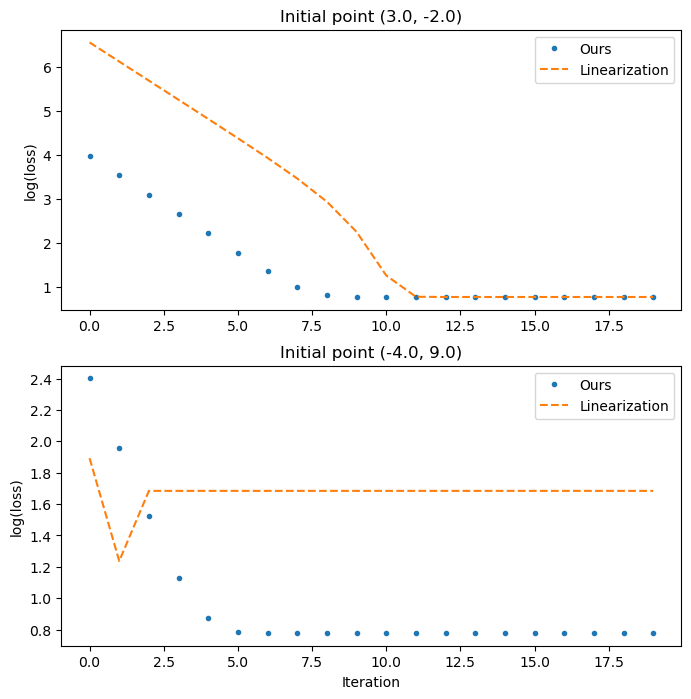
\includegraphics [scale=0.5]{./experiment/setting1.png}}
\caption{Experiment result of setting 1.}
\label{fig1}
\end{figure}

\begin{figure}[htbp]
\centerline{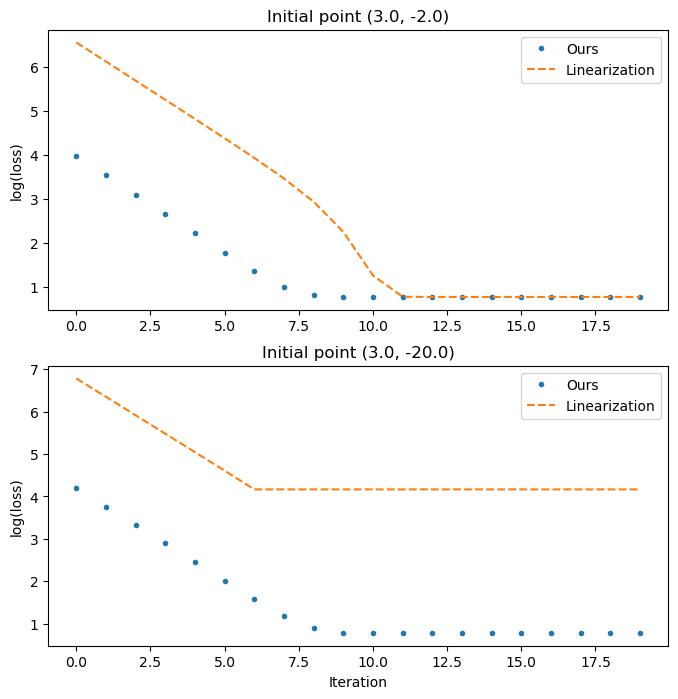
\includegraphics [scale=0.5]{./experiment/setting2.png}}
\caption{Experiment result of setting 2.}
\label{fig2}
\end{figure}

\begin{figure}[htbp]
\centerline{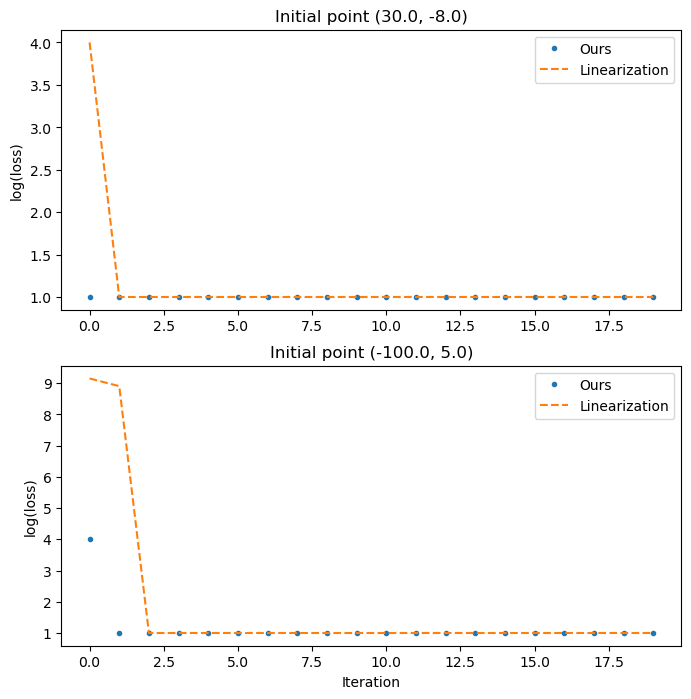
\includegraphics [scale=0.5]{./experiment/setting3.png}}
\caption{Experiment result of setting 3.}
\label{fig3}
\end{figure}

%--------------------------------------------------------------------------------
%Conclustion
\section{Conclusion}
In this report, we construct \textbf{Algorithm \ref{ouralg}} based on \textbf{Byzantine distributed optimization algorithm (BDOA)} \cite{liu2021approximate} and \textbf{Linearization}\cite{wilson2012linearization} for non-linear constraints optimization problem \eqref{P0}. 
The novelty of our algorithm is that we extend the definition of ``fault" in Byzantine distributed problem \eqref{bdop} and utilize BDOA as a filter. With the help of BDOA, in our algorithm, we can divide the constrained optimization problem \eqref{P0} into two parts, suitable for linear approximation or not. For the part suitable for linear approximation, we optimize it with linearization method; For the part unsuitable for linear approximation, we optimize it with \textbf{proximal point method}\cite{ppm}. Finally, we hybrid the above two parts with \textbf{proximal gradient method}\cite{pgm}. We expect our algorithm would be more efficient than linearization method for non-linear constrained optimization problem \eqref{P0}, since our algorithm can avoid the step size of liniearization method being too small due to unsuitable linear approximation.

Last but not least, we also perform a series of experiments to demonstrate the advantage of our algorithm. The experiments can be divided into three settings, exponential constraints, polynomial constraints, and ``exponential $+$ polynomial constraints" constraints. In all experiments, our algorithm shows a more efficient than linearization method.

In conclusion, in this report, we proposed \textbf{Algorithm \ref{ouralg}} which performs experimentally better compared to linearization method.

%-----------------------------------------------------------------------------
%Future works and unsolved problems
\section{Future works and unsolved problems}
There are still some topics that we could research in the future. The first one is the complexity of our algorithm. We have not given a theoretical proof to show our algorithm (\textbf{Algorithm \ref{ouralg}}) is better than linearization method. The obstacle for us to provide rigorous proof is that it is very hard to relate the complexity with `` unsuitable for linear approximation". We hope to prove that the complexity of our algorithm will be less than the complexity of linearization method, when the optimization problem which we consider is sufficiently unsuitable for linear approximation. However, we have no idea how to achieve our goal so far.
The second part is that we have not provided an estimation of hyper-parameters. In our algorithm, there are three hyper-parameters, $N_{\text{Filter}}$, $\alpha_2$, $k_{c}$. Sometimes, we need to spend some time on tuning these hyper-parameters in order to obtain better performance. To save time and make our algorithm more efficient for people, we still need to give an estimation of hyper-parameters.
The third part is that we want to do more experiments to demonstrate the feasibility of our algorithm. There are so many kinds of constraints we are interested in, but we do not have enough time to do experiments. 
Following is the list of future works mentioned above:
\begin{itemize}
    \item Provide theoretical proof to show our algorithm is better than linearization method,  when the optimization problem which we consider is sufficiently unsuitable for linear approximation.
    \item Provide an estimation of hyper-parameters.
    \item Do more experiments to show the feasibility of our algorithm.
\end{itemize}

%----------------------------------------------------------------------------------
%Reference
\bibliographystyle{ieeetr}
\bibliography{Ref}
\end{document}
